\documentclass{article}
\usepackage{cancel}
\usepackage{amsmath, amssymb, amsfonts}
\usepackage[binary-units]{siunitx}
\usepackage{tikz}
\usepackage{float}
\usepackage{pgffor}
\usepackage{import}
\usepackage{vwcol}
\usepackage{fontawesome}
\usepackage{stmaryrd}
\usepackage{multicol}
\usepackage{pdfpages}
\usepackage{transparent}
\usepackage{xcolor}
\usepackage{scalerel}
\usepackage{stackengine}
\usepackage{algpseudocode}
\newcommand{\diag}{\operatorname{diag}}
\newcommand{\card}{\operatorname{card}}
\newcommand{\tr}{\operatorname{tr}}
\newcommand{\rg}{\operatorname{rg}}
\renewcommand{\epsilon}{\varepsilon}
\newcommand{\equivalent}[1]{\underset{#1}{\sim}}
\newcommand{\R}{\mathbb{R}}
\newcommand{\Q}{\mathbb{Q}}
\newcommand{\C}{\mathbb{C}}
\newcommand{\N}{\mathbb{N}}
\newcommand{\Z}{\mathbb{Z}}
\newcommand{\cM}{\mathcal{M}}
\newcommand{\cO}{\mathcal{O}}
\newcommand{\dx}{\mathrm{d}x}
\newcommand{\dy}{\mathrm{d}y}
\newcommand{\dz}{\mathrm{d}z}
\newcommand{\dt}{\mathrm{d}t}
\newcommand{\df}{\mathrm{d}f}
\newcommand{\Sp}{\operatorname{Sp}}
\newcommand{\dangersign}[1][2ex]{%
  \renewcommand\stacktype{L}%
  \scaleto{\stackon[1.3pt]{\color{red}$\triangle$}{\tiny !}}{#1}%
}

\usepackage[a4paper,top=4cm,bottom=4cm,left=3cm,right=3cm,marginparwidth=1.75cm]{geometry}
% \newcommand{\incfig}[2][1]{%
%     \def\svgwidth{#1\columnwidth}
%     \import{./figures/}{#2.pdf_tex}
% }
% 
\newenvironment{theorem}[1][\unskip]{
	\paragraph{Théorème #1}

}{}

\newenvironment{proof}[1][\unskip]{
	\def\temp{#1}\ifx\temp\empty
		\paragraph{Preuve}
	\else
		\paragraph{Preuve \emph{(#1)}}
	\fi

}{}

\newenvironment{definition}[1][\unskip]{
	\paragraph{Définition: #1}

}{}

\newenvironment{warning}[1][\unskip]
{
	\vspace{1cm}
	\begin{minipage}[c]{0.1\linewidth}
	\dangersign[8ex] 
\end{minipage}%
\begin{minipage}[l]{0.9\linewidth}
}
{
	\end{minipage}
	\vspace{1cm}
}

% \pdfsuppresswarningpagegroup=1


\begin{document}
\section{Comparaison de systèmes de transmission sur fréquence porteuse}

\subsection{}
Fréquence porteuse

\subsection{}


\begin{figure}[H]
    \centering
    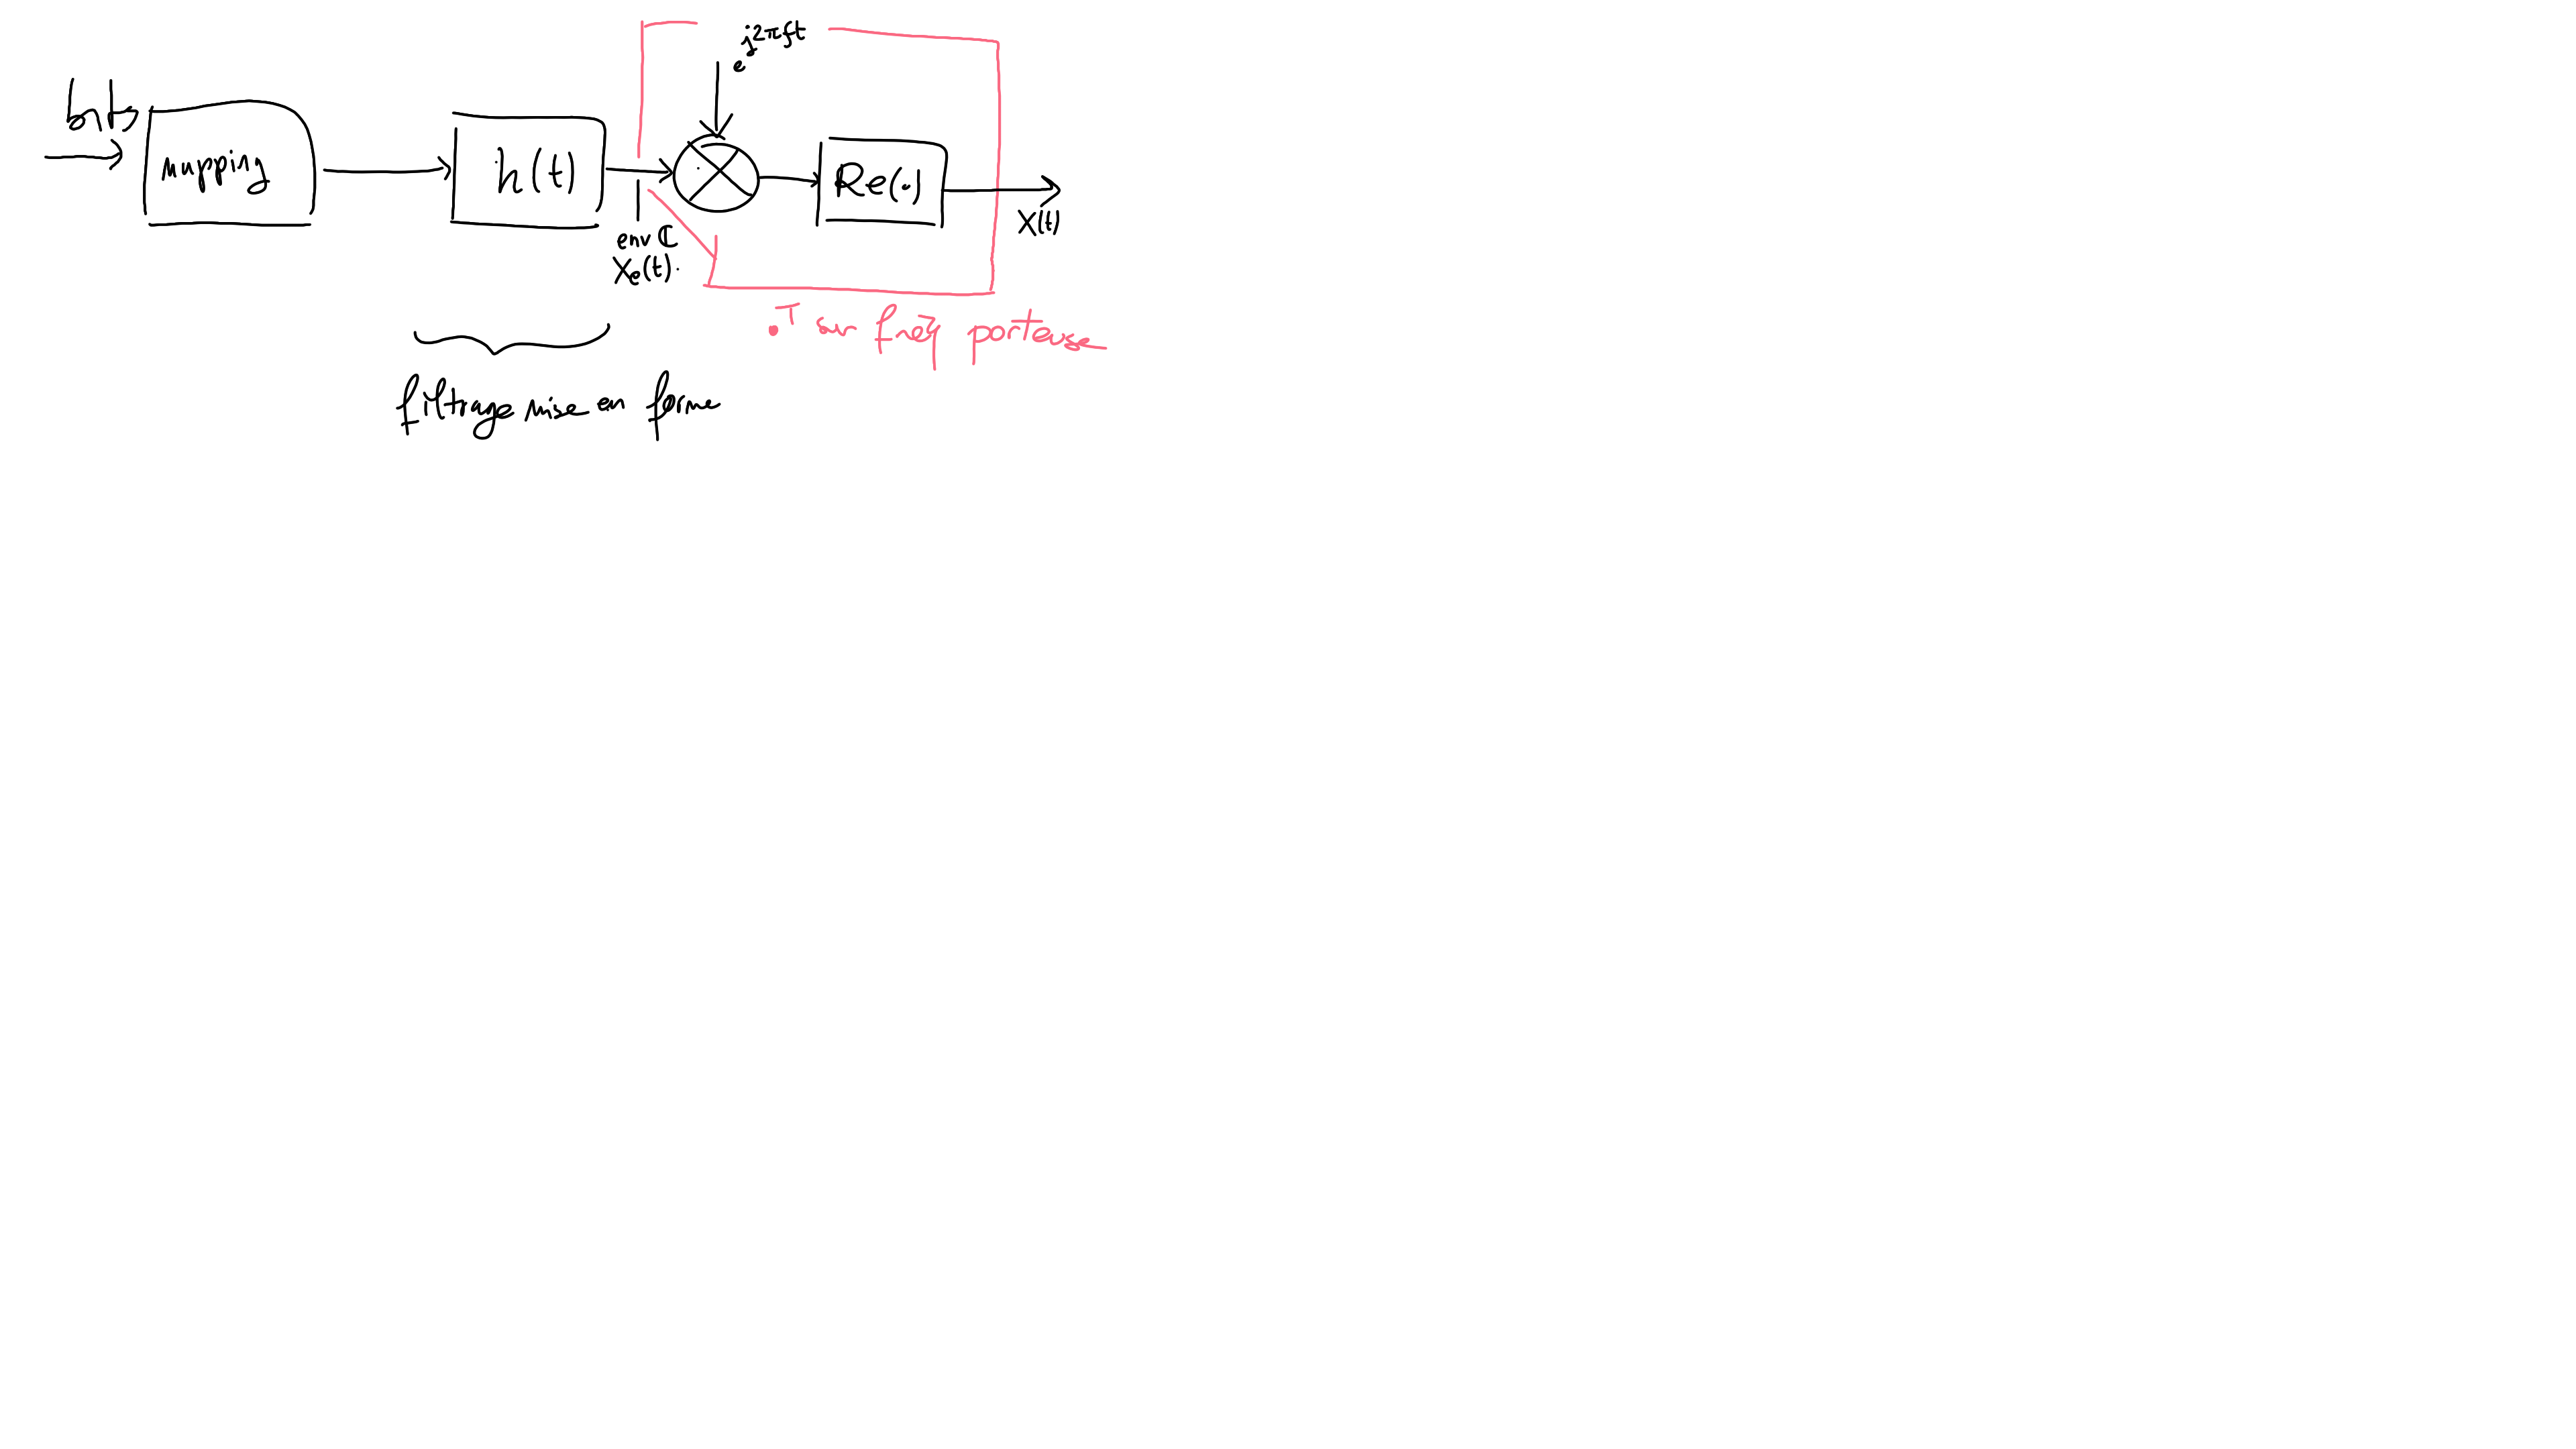
\includegraphics[width=0.8\textwidth]{1.2.png}
    \caption{}
    \label{fig:}
\end{figure}

\paragraph{Remarque}

\begin{align*}
    X(t) = \Re X_e(t) e^{2j \pi f_0 t}
    &= \underbrace{\Re X_e(t)}_{I(t)} \cos(2 \pi f_0 t) - \underbrace{\Im X_e(t)}_{Q(t)} \sin(2 \pi f_0 t) \\
\end{align*}

Avec $X_e = I + Q$ ($I$ pour \emph{en phase } et $Q$ pour \emph{en quadrature})

\subsection{}
L'ordre est de 4 dans les 3 cas.

\subsection{}
\begin{figure}[H]
    \centering
    \includegraphics[width=0.8\textwidth]{1.4.png}
    \caption{}
    \label{fig:}
\end{figure}

\subsection{}
$$R_s = \frac{R_b}{\log_2(16)} = \frac{R_b}{4}$$
\subsection{}


\begin{align*}
    \eta &= \frac{R_b}{B} \\
\end{align*}

avec $B$ la bande passante

Ici, on a une racine de  cosinus surélevé, donc $B = (1+\alpha) R_s$

\begin{figure}[H]
    \centering
    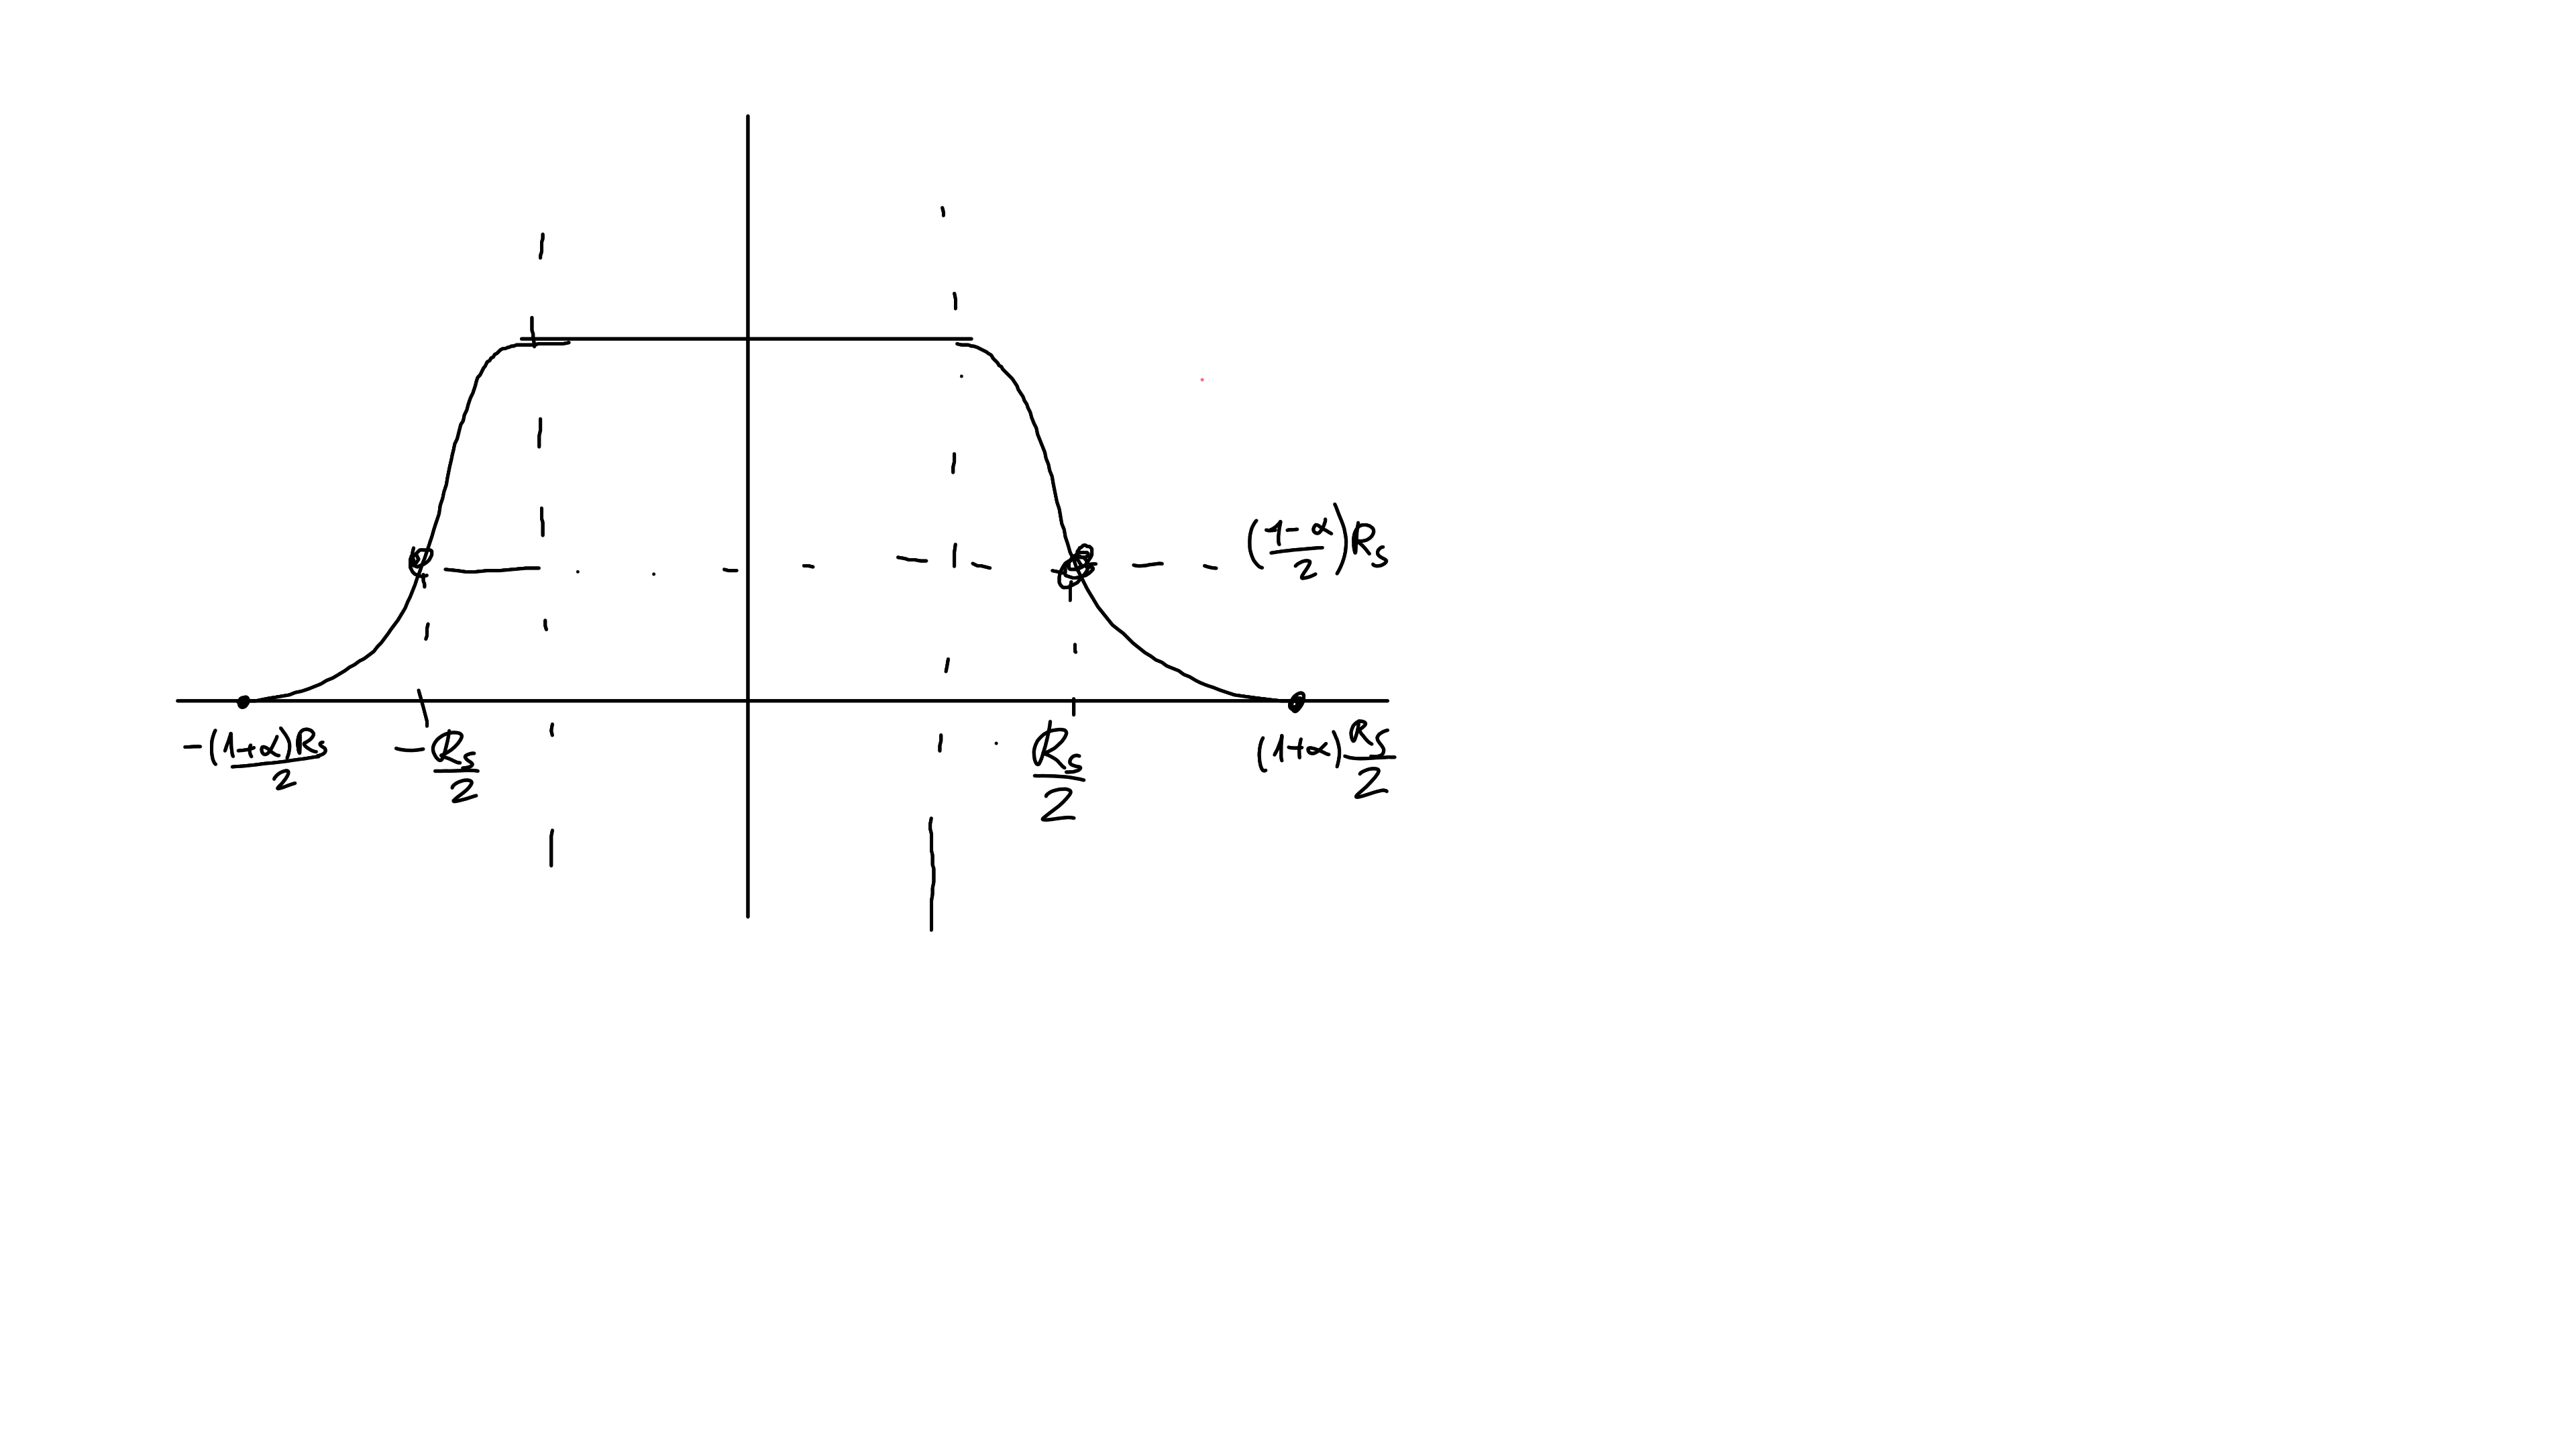
\includegraphics[width=0.8\textwidth]{1.6.png}
    \caption{1}
    \label{fig:1}
\end{figure}

\paragraph{Application numérique} avec $\alpha = 0.5, M = 16$

\begin{align*}
    \eta = \frac{4}{1,5} = \SI{8 / 3}{b s^{-1} Hz^{-1}}
\end{align*}

\subsection{}
On a $\argmax_\alpha \eta(\alpha) = 0$. Donc $\max \eta = \SI{4}{b s^{-1} Hz^{-1}}$.

Ainsi $B = (1+\alpha) R_s = \SI{12}{kHz}$ 




\end{document}
